\documentclass[11pt]{beamer}
\usepackage[utf8]{inputenc}
\usepackage[T1]{fontenc}
\usepackage{lmodern}
\usetheme{default}
	\usefonttheme[onlymath]{serif}

\usepackage{graphicx}
	\graphicspath{{Pictures/}}
\usepackage{subfig}
\captionsetup[subfloat]{labelformat=empty}
\captionsetup[figure]{labelformat=empty}

\usepackage{booktabs} % per le tabelle, permette di usare \toprule ecc
\usepackage{amsmath}
\usepackage{mathtools}
\usepackage{multimedia}
\usepackage{hyperref}
\usepackage{ifxetex}
\ifxetex
	\usepackage{fontspec}
	\setsansfont[Scale=0.95]{Arial}
\fi

\setbeamertemplate{footline}[frame number]

\begin{document}
	\author{Alessio Raimondi}
	\title{Literature review on non-spherical particles}
	%\subtitle{}
	%\logo{}
	%\institute{}
	%\date{}
	%\subject{}
	%\setbeamercovered{transparent}
	%\setbeamertemplate{navigation symbols}{}
	\begin{frame}[plain]
		\maketitle
	\end{frame}
	
%	\begin{frame}
%		\centering
%		\includegraphics[height=\textheight,width=\textwidth,keepaspectratio]{LiteratureReview.png}		
%	\end{frame}

%	\begin{frame}
%		\begin{columns}[T]
%			\begin{column}
%				"Old":\\
%				\begin{itemize}
%					\item Haider & Levenspiel - 1989
%					\item Hartman - 1994
%					\item Chien - 1994
%					\item Swamme & Ojha - 1991
%				\end{itemize}
%			\end{column}
%			\begin{column}
%				"New":\\
%				\begin{itemize}
%					\item Ganser - 1993
%					\item Holzer & Sommerfeld - 2008
%					\item Tran, Cong et al. - 2004
%					\item Loth - 2008
%				\end{itemize}
%			\end{column}
%		\end{columns}
%	\end{frame}

	\begin{frame}{Drag curves - all models}
		\centering
		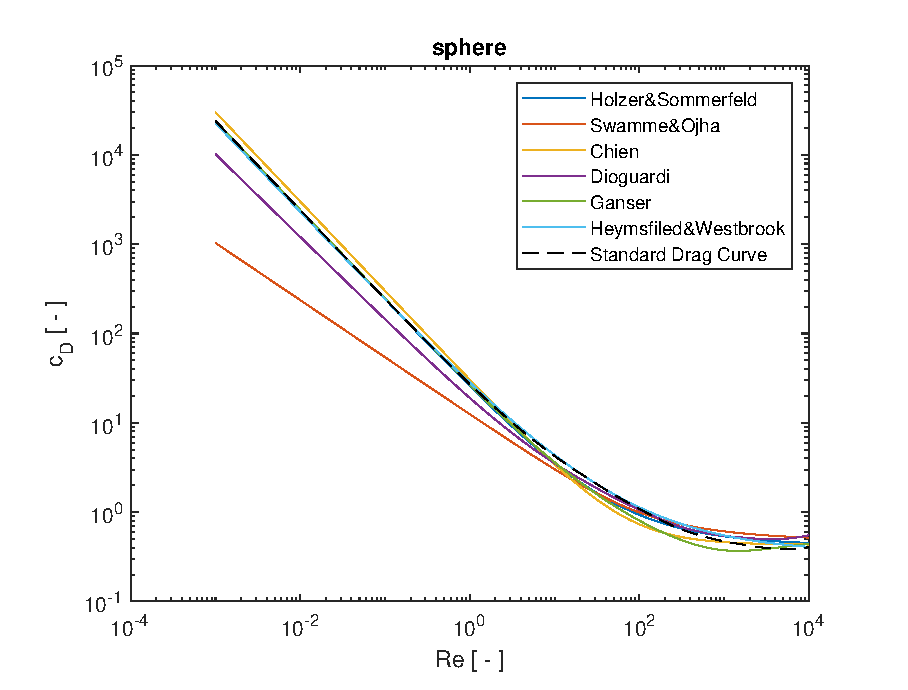
\includegraphics[height=\textheight,width=\textwidth,keepaspectratio] {sphere_cD_all.eps}		
	\end{frame}

	\begin{frame}{Chhabra, Agarwal, Sinha - 1998}
		Critical review of a selection of widely used correlation formulae for the estimation of $ c_D $ of non-spherical particles in incompressible viscous flow.
		\begin{itemize}
			\item \textbf{Data points:} 1900
			\item \textbf{Sphericity:} 0.09 - 1
			\item \textbf{Re:} $ 10^{-4} - 5 \cdot 10^5 $
			\item \textbf{Methods analyzed:} Ganser [1993], Haider and Levenspiel [1989], Hartman [1994], Chien [1994] and Swamme and Ojha [1991] - Ordered by decreasing performance.
		\end{itemize}
	\end{frame}

	\begin{frame}{Chhabra, Agarwal, Sinha - 1998}
		Conclusions:
		\begin{itemize}
			\item \textbf{Reference length:} equal volume sphere diameter $ d_{\textup{v}} = \sqrt{\dfrac{6 V}{\pi}} $
			\item \textbf{Shape parameter:} Swamme and Ojha uses the \textit{Corey shape factor} ($ \beta $) while the other four uses the \textit{Sphericity} $ \Phi $
			\item \textbf{Swamme and Ojha} Poor prediction (only one set of data was used), valid only for $ Re > 1 $.
			\item \textbf{Ganser:} Best overall method if Lasso and Weideman's results are not taken into account (hollow cylinder and agglomerates made of spherical particles). It's the only one that takes in consideration the \textbf{orientation of the particle}.\\
			Nb. After Chhabra's review, this will be a minimum requisite for a drag model.
		\end{itemize}
	\end{frame}

	\begin{frame}{Symbols}
		\begin{tabular}{ccl}
			$ d_{\textup{v}} $ & & diameter of the sphere with equivalent volume \\
			\\
			$ d_{\textup{n}} $ & & diameter of the sphere with equivalent projected area\\
			\\
			$ d_{\textup{s}} $ & & diameter of the sphere with equivalent surface area\\
			\\
			$ d_{\textup{c}} $ & & diameter of the circumscribing circle\\
			\\
			$ A_{\textup{p}} $ & & area of the particle
		\end{tabular}
	\end{frame}

	\begin{frame}{Ganser - 1993}
		\begin{equation*}
		c_D = K_2 \frac{24}{Re K_1 K_2} (1 + 0.1118 (Re K_1 K_2)^{0.6567}) + \frac{0.4305}{1 + \frac{3305}{Re K_1 K_2}}
		\end{equation*}
		\begin{itemize}
			\item Function of the generalized Reynolds number ($ Re K_1 K2 $) only!
		\end{itemize}
		\vfill
		Comes from empirical correlations of the general drag formula by \textit{Haider and Levenspiel (1989)}:
		\begin{equation*}
		c_D = \frac{24}{Re} (1 + A Re^B) + \dfrac{C}{1 + \frac{D}{Re}}
		\end{equation*}
	\end{frame}
	
	\begin{frame}{Ganser - 1993}
		\begin{block}{Stokes' shape factor}
			\begin{equation*}
			K_1 = \left( \frac{1}{3} \frac{d_n}{d_v} + \frac{2}{3} \Phi^{-\frac{1}{2}} \right)^{-1} -2.25 \frac{d_v}{D_{\textup{tube}}} 
			\end{equation*}
		\end{block}
		\begin{block}{Newton's shape factor}
			\begin{equation*}
			K_2 = 10^{1.8148 (-log(\Phi))^{0.5743}}
			\end{equation*}
		\end{block}
	\end{frame}

	\begin{frame}{Symbols}
		\begin{block}{Sphericity}
			\begin{columns}[T]
				\begin{column}{.4\textwidth}
					\begin{equation*}
					\Phi = \dfrac{\pi \ d_{\textup{v}}^2} {A_{\textup{p}}}
					\end{equation*}
				\end{column}
				
				\begin{column}{.6\textwidth}
					Ratio between the surface area of the volume-equivalent sphere and the area of the actual particle
				\end{column}
			\end{columns}
		\end{block}
		\vfill
		\begin{block}{Crosswise Sphericity}
			\begin{columns}[T]
				\begin{column}{.4\textwidth}
					\begin{equation*}
					\Phi_{\perp} = \dfrac{\frac{\pi}{4}\ d_{\textup{v}}^2} {A_{\textup{p}, \perp}}
					\end{equation*}
				\end{column}
				
				\begin{column}{.6\textwidth}
					Ratio between the cross-sectional area of the volume-equivalent sphere and the projected cross-sectional area of the actual particle
				\end{column}
			\end{columns}
		\end{block}
	\end{frame}
	
	\begin{frame}{Symbols}
		\begin{block}{Lengthwise Sphericity}
			\begin{columns}[T]
				\begin{column}{.4\textwidth}
					\begin{equation*}
					\Phi_{/\!/} = \dfrac{\frac{\pi}{4}\ d_{\textup{v}}^2} {\Delta A}
					\end{equation*}	
					\vfill		
					\begin{equation*}
					\Delta A = \dfrac{A_{\textup{p}}}{2} - \bar{A_{\textup{p},/\!/}}
					\end{equation*}
				\end{column}
				
				\begin{column}{.6\textwidth}
					Ratio between the cross-sectional area of the volume-equivalent sphere and the difference between half the surface area and the mean longitudinal projected cross-sectional area of the actual particle.\\
					Since $ A_{\textup{particle},/\!/} $ depends on the angle of view, an arithmetic average over an entire revolution is used
				\end{column}
			\end{columns}
		\end{block}
	\end{frame}

	\begin{frame}{Holzer and Sommerfeld - 2008}
		\begin{itemize}
			\item Huge literature and data review (2061 values)
			\item Interpolation of different previous models
			\item Arbitrary shape (and Orientation!)
			\item Valid for all the Subcritical Regime
		\end{itemize}
	
		\begin{equation*}
			c_D = \frac{8}{Re} \frac{1}{\sqrt{\Phi_{/\!/}}} + \frac{16}{Re} \frac{1}{\Phi} + \frac{3}{\sqrt{Re}} \frac{1}{\Phi^{\frac{3}{4}}} + 0.4210^{0.4(-\log \Phi)^{0.2}} \frac{1}{\Phi_{\perp}}
		\end{equation*}
	\end{frame}

%	\begin{frame}{Holzer and Sommerfeld - 2008}
%		\includegraphics[width=\linewidth]{ComparisonH&S.png}
%		\begin{itemize}
%			\item Works better than the other for disks and plates
%			\item Ganser works better for isometric particles
%			\item Works well overall
%		\end{itemize}
%	\end{frame}
%
%	\begin{frame}{Sanjeevi, Padding and Kuipers -- 2015}
%		DNS of a prolate Ellipsoid with $ \Phi = 0.886 $
%		\centering
%		\includegraphics[height=.8\textheight]{DNS.png}
%	\end{frame}

	\begin{frame}{Stokes Regime}
		\begin{equation*}
			c_D = \frac{8}{Re} \frac{1}{\sqrt{\Phi_{\perp}}} + \frac{16}{Re} \frac{1}{\Phi}
		\end{equation*}
		\vfill
		\begin{itemize}
			\item Leith's model - 1993
			\item Valid for low Re ($\leq 10$)
			\item For sphere ($ \Phi_{\perp} = \Phi_{/\!/} = \Phi $) degenerates to Stokes' analytical solution
			\item Modification: $ \Phi_{\perp} \rightarrow \Phi_{/\!/} $   (for better approximation of the $ c_D $ as a function of the particle orientation)
		\end{itemize}
	\end{frame}

	\begin{frame}{Newton Regime}
		\begin{block}{Blasius - 1908}
			Friction drag for plates and disks (small cross-sectional area)
			\begin{equation*}
				c_D = 1.327 \cdot 2 \left(\frac{8}{9}\right)^{\frac{1}{4}} \pi^{\frac{1}{4}} \left(\frac{\text{depth}}{\text{length}}\right)^{\frac{1}{4}} \frac{1}{\Phi^{\frac{3}{4}}} \frac{1}{\sqrt{Re}}
			\end{equation*}
			for square plates: \quad $ c_D = 3.43 / (\Phi^{\frac{3}{4}} \sqrt{Re}) $
		\end{block}
	
		\begin{block}{Tran-Cong (2004) and Ganser (1993)}
			Term for high Re proportional to the projected cross-sectional area (Tran-Cong) with the same factor of proportionality of Ganser.
			\begin{equation*}
				c_D = 0.4210^{0.4(-\log \Phi)^{0.2}} \frac{1}{\Phi_{\perp}}
			\end{equation*}
		\end{block}
	\end{frame}

	\begin{frame}{Heymsfield and Westbrook - 2010}
		Adjustment of the Mitchell's (1996) formula (sphere drag model with altered coefficients)
		\begin{equation*}
			c_D = C_0 \left( 1 + \frac{\delta_0}{\sqrt{Re}} \right)^2
		\end{equation*}
		by means of the area ratio $ A_r $ in order to fit more geometries:
		\begin{equation*}
			c_D^* = c_D \ A_r^k = 0.35 \left( 1 + \frac{8}{\sqrt{Re}} \right)^2 A_r^{0.5}
		\end{equation*}
		\begin{itemize}
			\item Only artificial ice shapes used to compute the model equation: planar crystals (List and Schemenauer - 1971) and spherical aggregates (Tran, Cong et al. - 2004)
			\item Oversensitivity to $ A_r $ of the formula for small area ratio (0.2-0.4)
		\end{itemize}
	\end{frame}
	

	\begin{frame}
		\begin{block}{Area ratio}
			\vfill
			\begin{columns}[T]
				\begin{column}{.4\textwidth}
					\begin{equation*}
					A_r = \dfrac{A_{\textup{p}, \perp}}{\frac{\pi}{4}\ d_{\textup{c}}^2}
					\end{equation*}	
				\end{column}
				
				\begin{column}{.6\textwidth}
					Ratio between the projected cross-sectional area of the actual particle and the area of the circumscribing circle
				\end{column}
			\end{columns}
		\end{block}
	\end{frame}
	
	\begin{frame}{Experimental data}
		\centering
		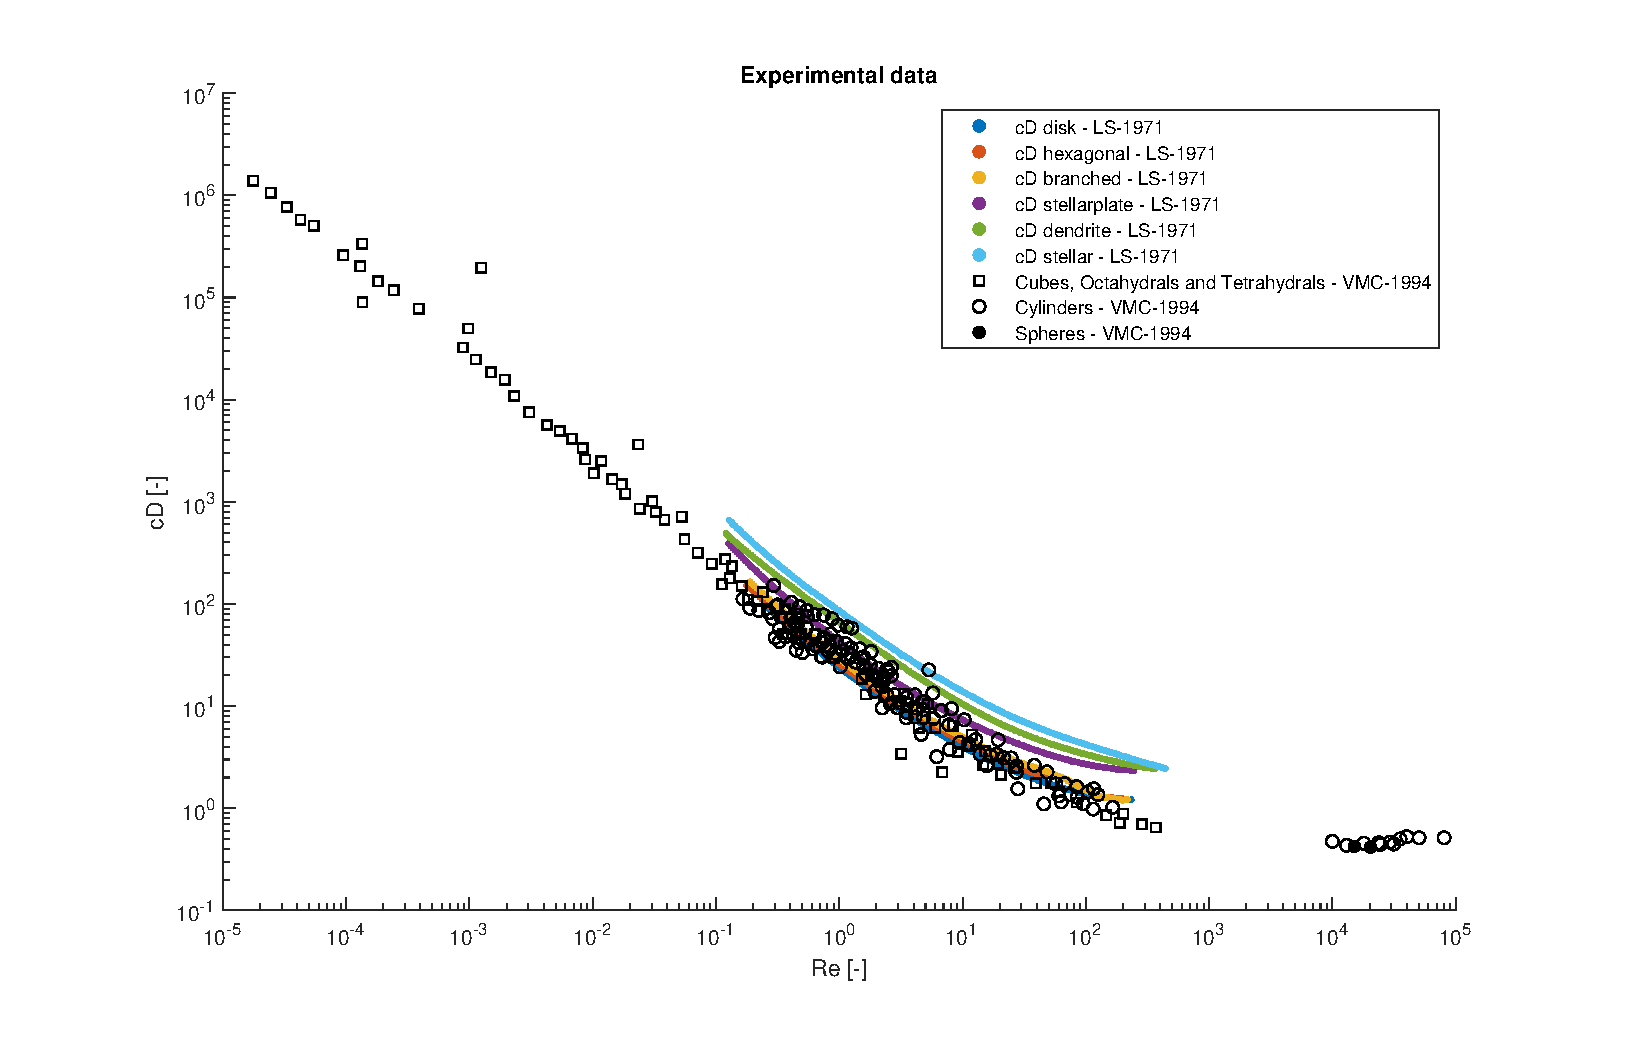
\includegraphics[height=\textheight,width=\textwidth,keepaspectratio] {exp_data.eps}		
	\end{frame}
	
	\begin{frame}{Drag curves - comparison}
		\centering
		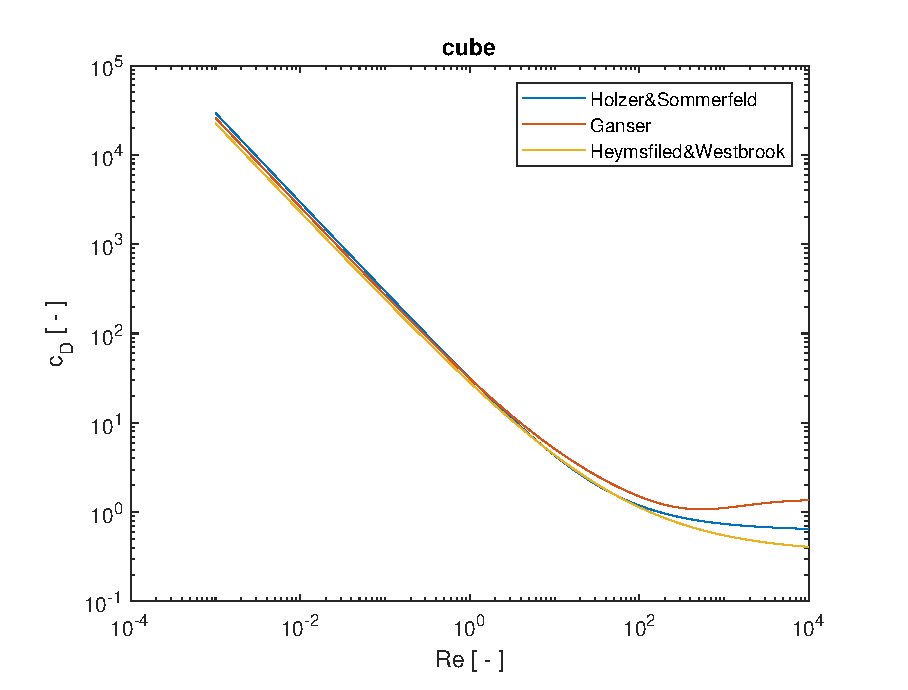
\includegraphics[height=\textheight,width=\textwidth,keepaspectratio] {cube_cD.eps}		
	\end{frame}

	\begin{frame}{Drag curves - comparison}
		\centering
		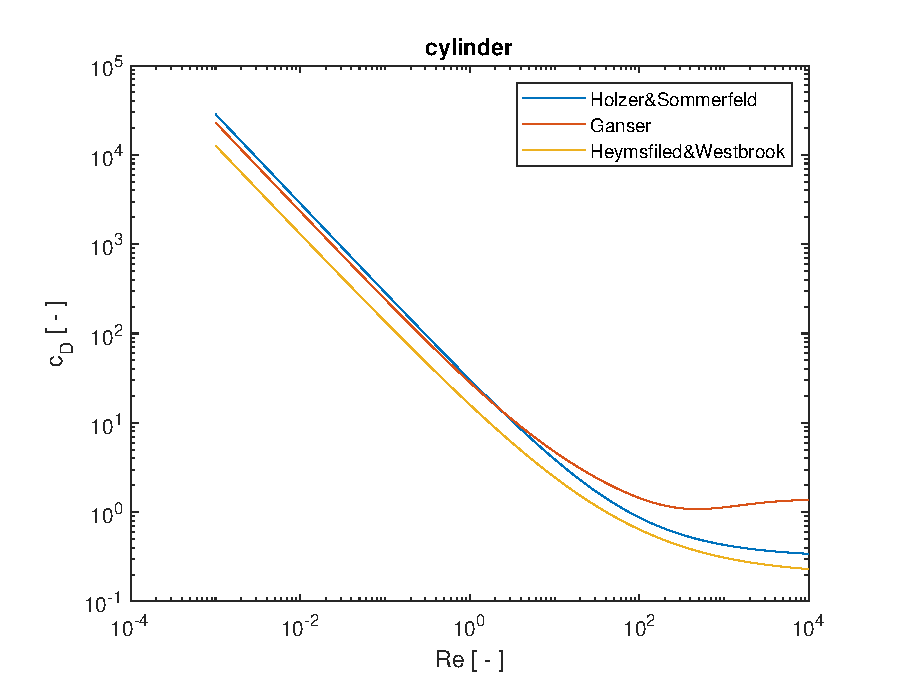
\includegraphics[height=\textheight,width=\textwidth,keepaspectratio] {cylinder_cD.eps}		
	\end{frame}

	\begin{frame}{Terminal Velocity}
		General equation:
		\begin{equation*}
			\frac{1}{2} \rho_{f}\ v_{lim}^2\ S_p\ c_D(Re(v_{lim}), model, shape) = W - F_b
		\end{equation*}
		becomes
		\begin{equation*}
			v_{lim}^2\ c_D(Re(v_{lim}, d_{\textup{v}}), model, shape) = \frac{4}{3} \dfrac{\rho_{p} - \rho_{f}}{\rho_{f}}\ g \ d_{\textup{v}}
		\end{equation*}
		and is solved iteratively for the unknown $ v_{lim} $, where $ d_{\textup{v}} $ is the independent variable and \textit{model} and \textit{shape} are parameters.
	\end{frame}

	\begin{frame}{References}
		\centering
		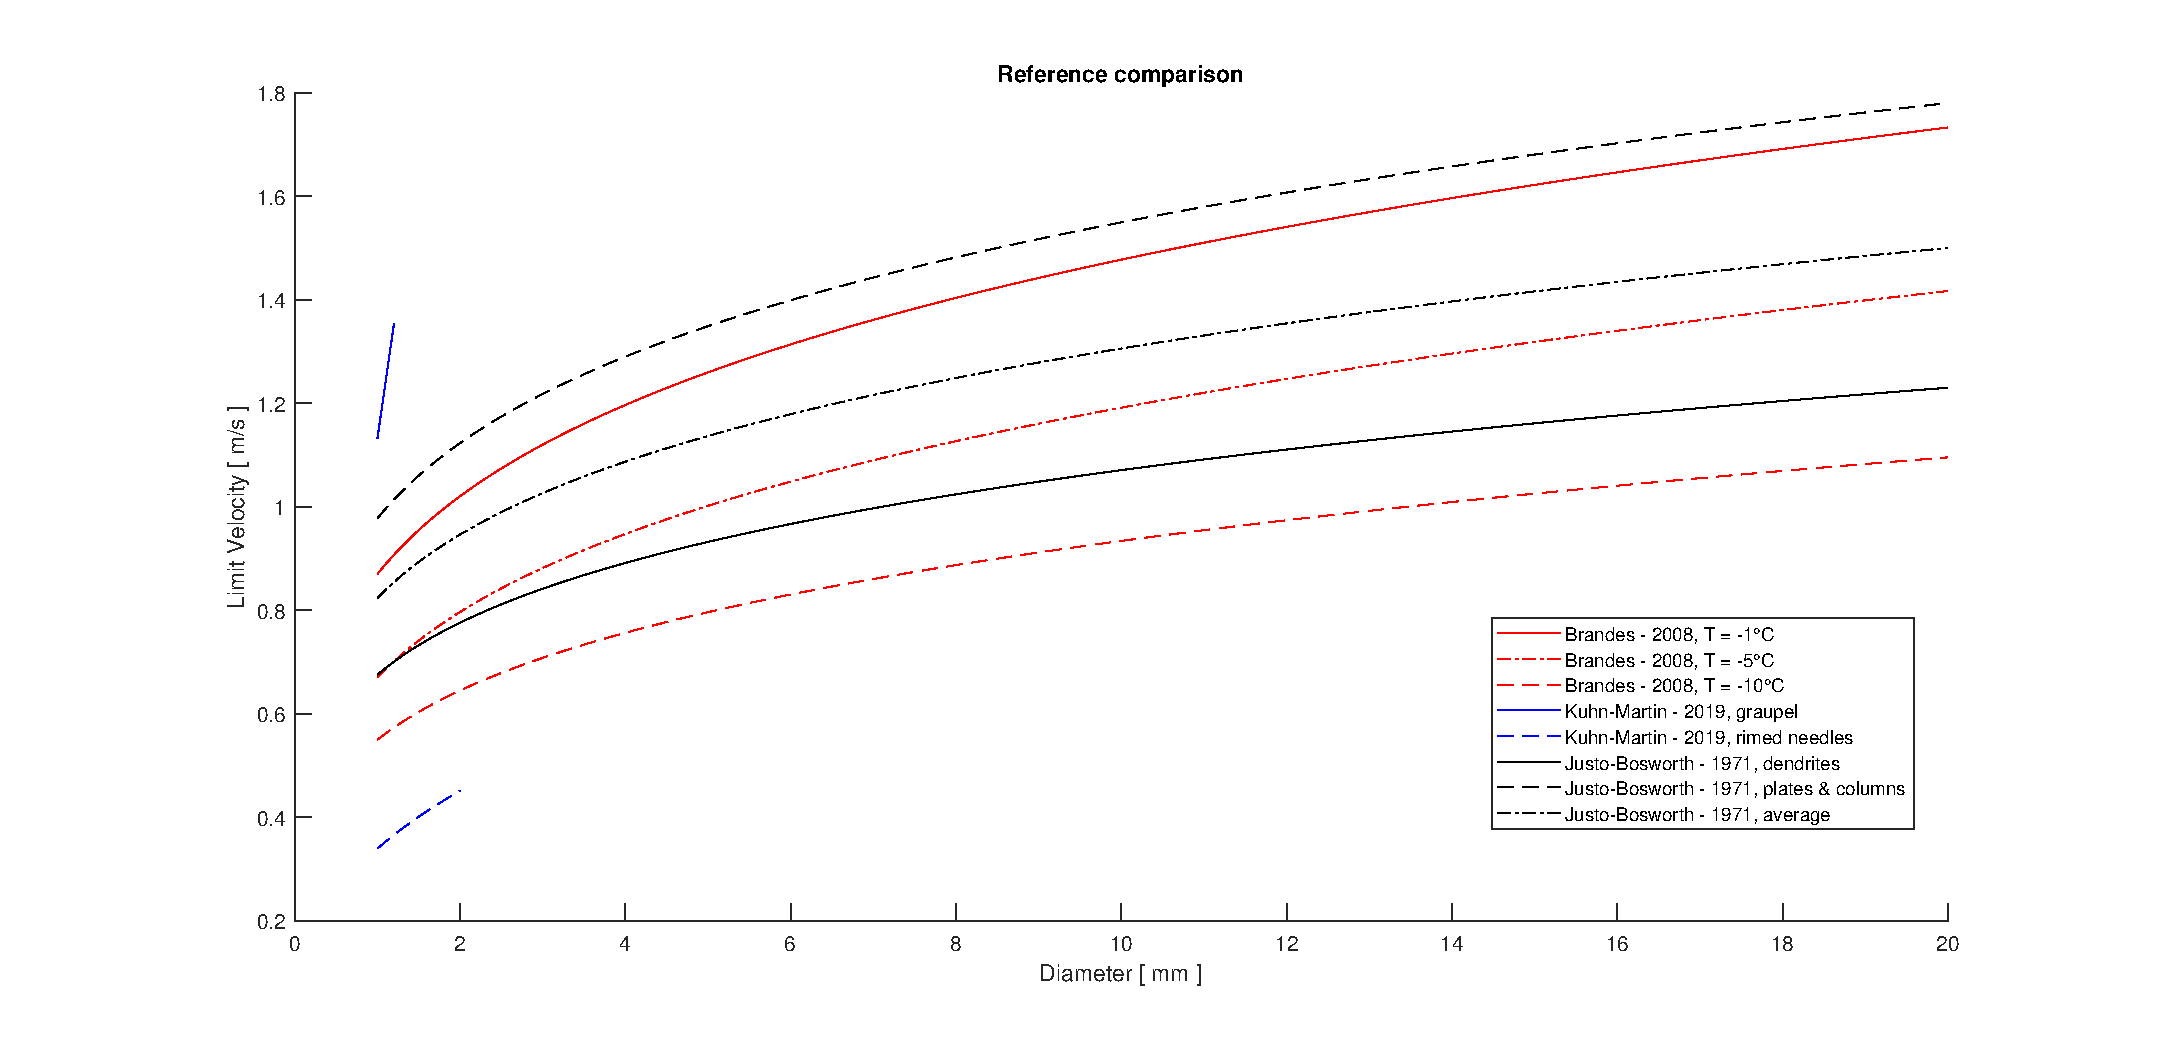
\includegraphics[height=\textheight,width=\textwidth,keepaspectratio] {references_vt_all.eps}		
	\end{frame}

	\begin{frame}{Unicity of the solution (1/2)}
		\centering
		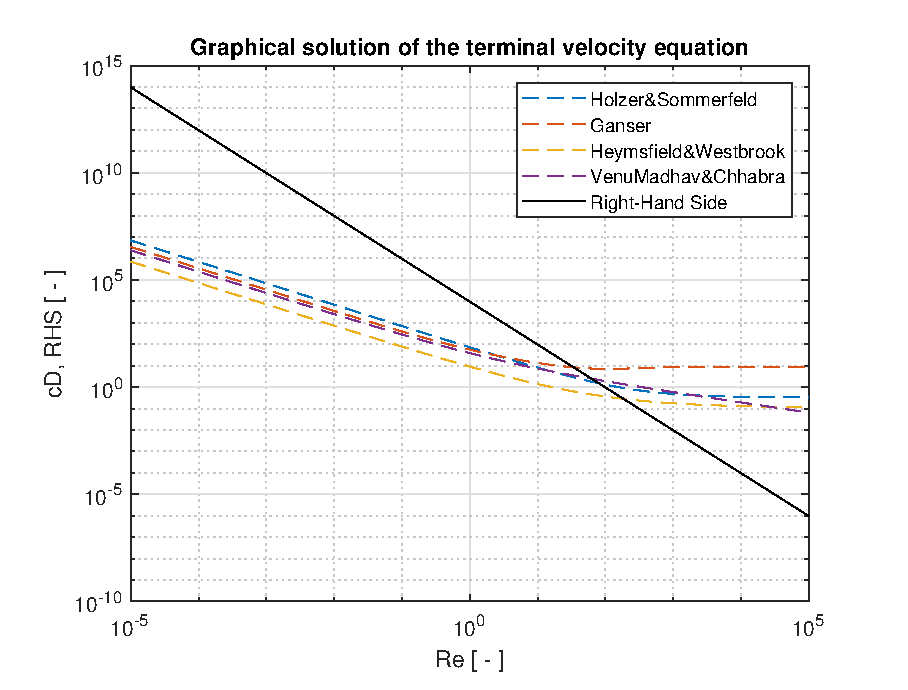
\includegraphics[height=\textheight,width=\textwidth,keepaspectratio] {unicity_min.eps}		
	\end{frame}

	\begin{frame}{Unicity of the solution (2/2)}
		\centering
		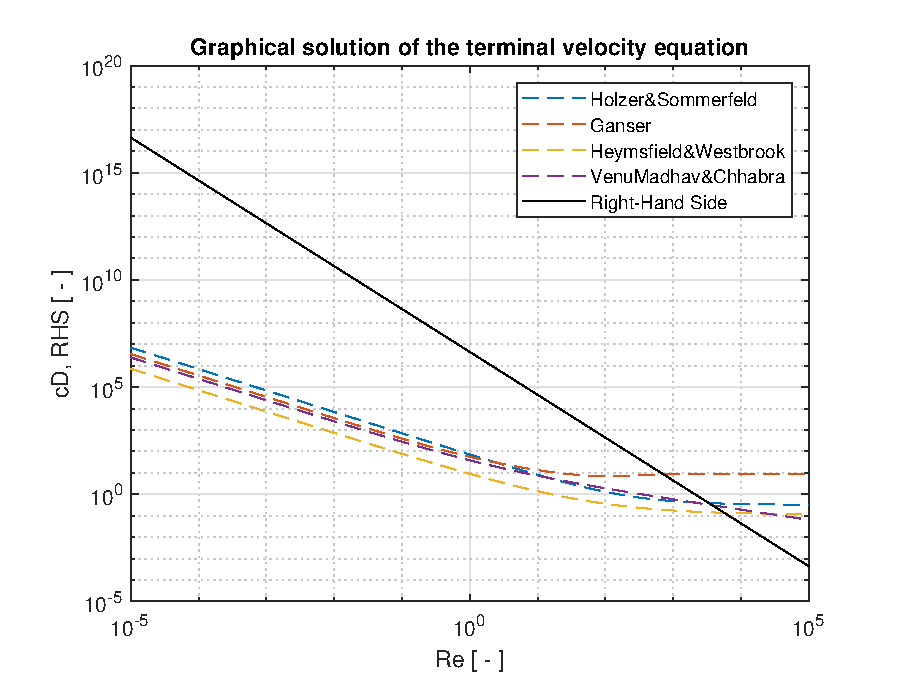
\includegraphics[height=\textheight,width=\textwidth,keepaspectratio] {unicity_max.eps}		
	\end{frame}

	\begin{frame}{Terminal velocity - comparison}
		\centering
		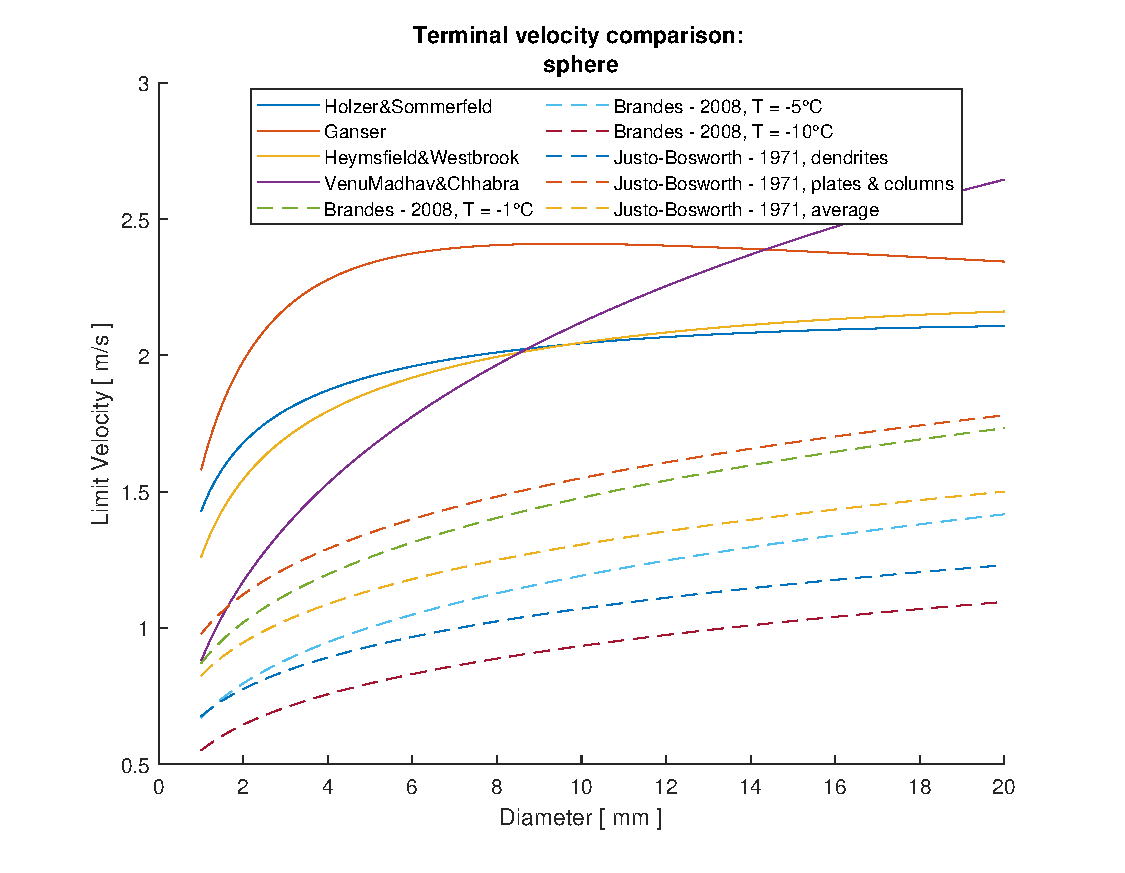
\includegraphics[height=\textheight,width=\textwidth,keepaspectratio] {vt_sphere.eps}		
	\end{frame}

	\begin{frame}{Terminal velocity - comparison}
		\centering
		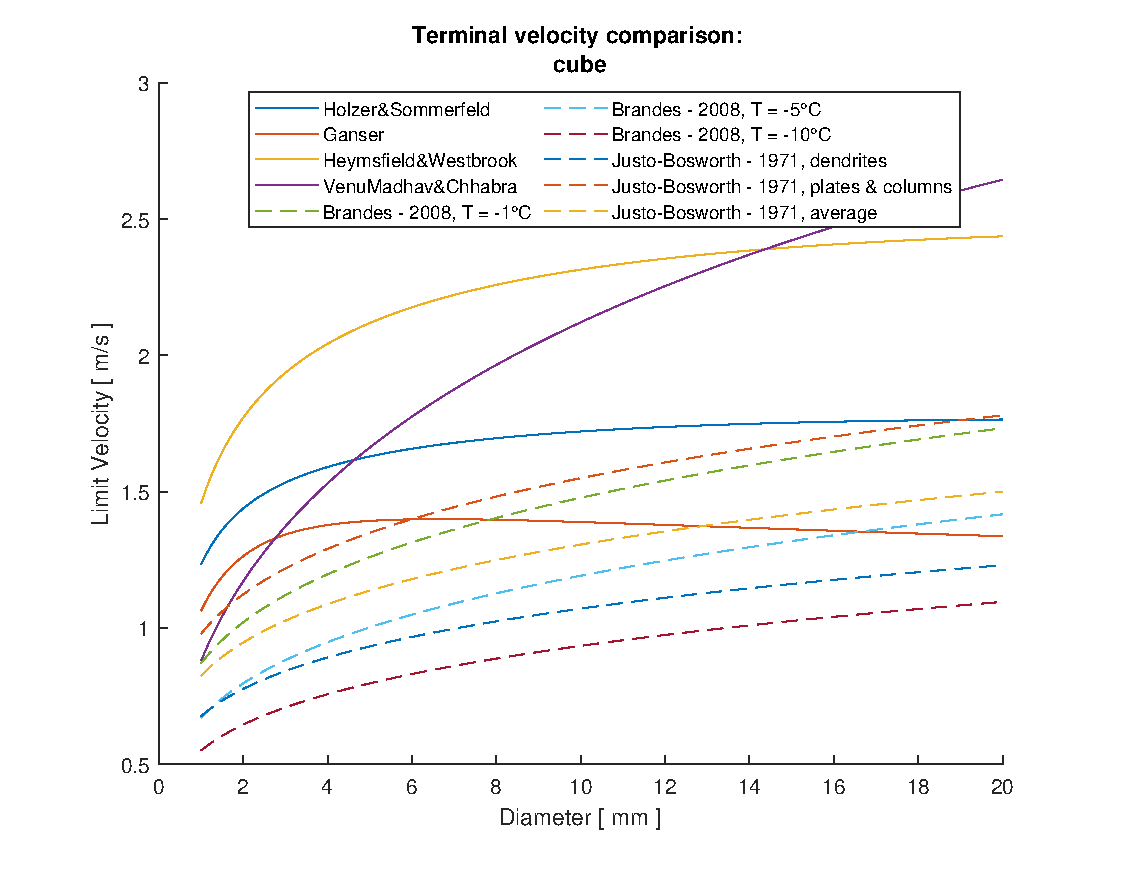
\includegraphics[height=\textheight,width=\textwidth,keepaspectratio] {vt_cube.eps}		
	\end{frame}

	\begin{frame}{Terminal velocity - comparison}
		\centering
		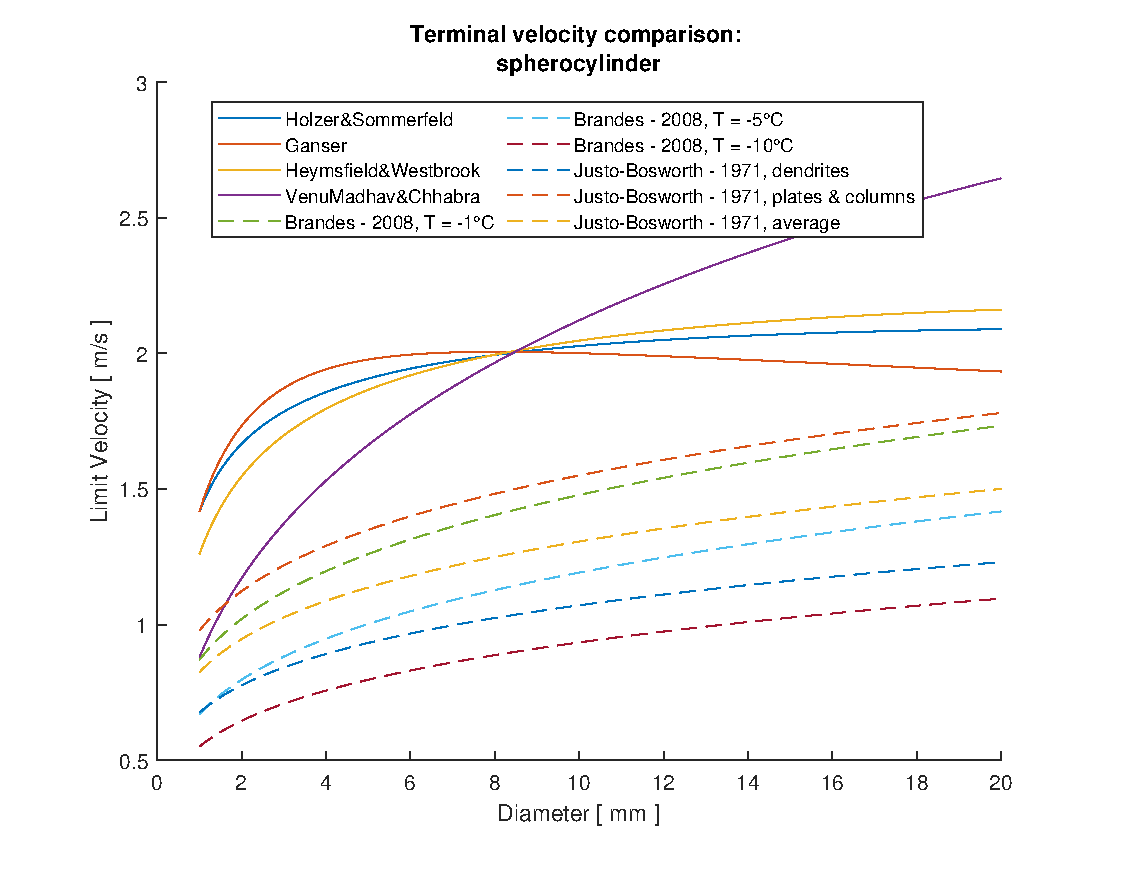
\includegraphics[height=\textheight,width=\textwidth,keepaspectratio] {vt_spherocylinder.eps}		
	\end{frame}

	\begin{frame}{Terminal velocity - comparison}
		\centering
		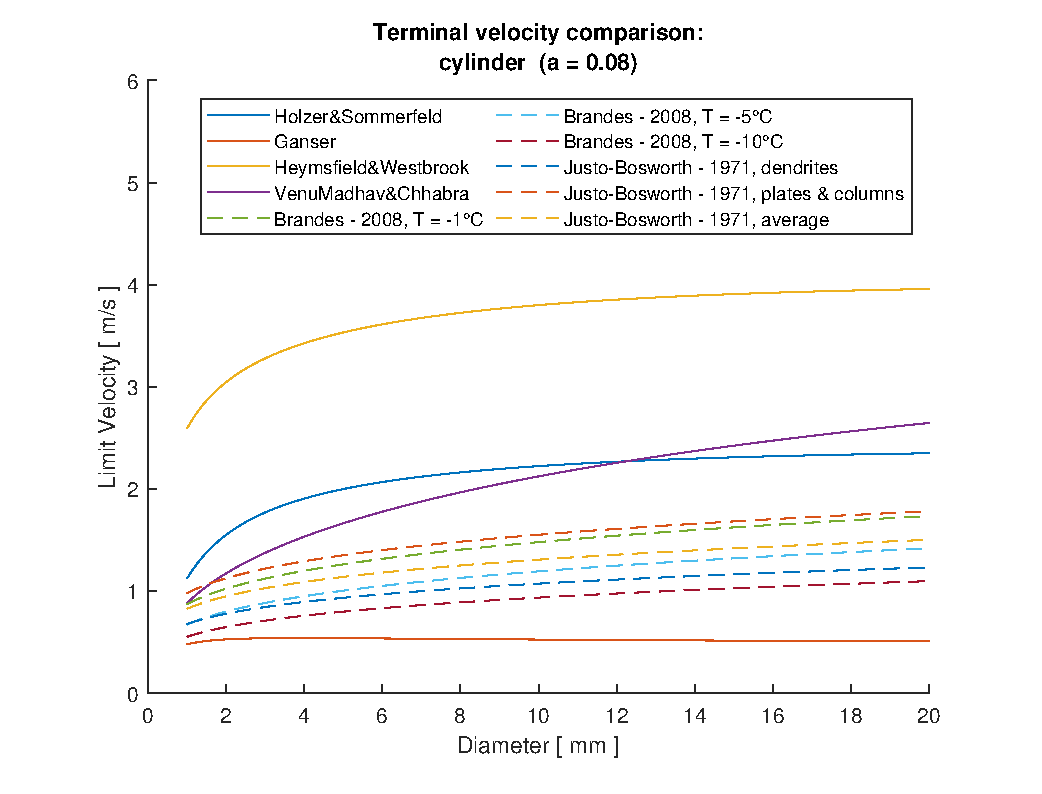
\includegraphics[height=\textheight,width=\textwidth,keepaspectratio] {vt_cylinder008.eps}		
	\end{frame}

	\begin{frame}{Terminal velocity - comparison}
		\centering
		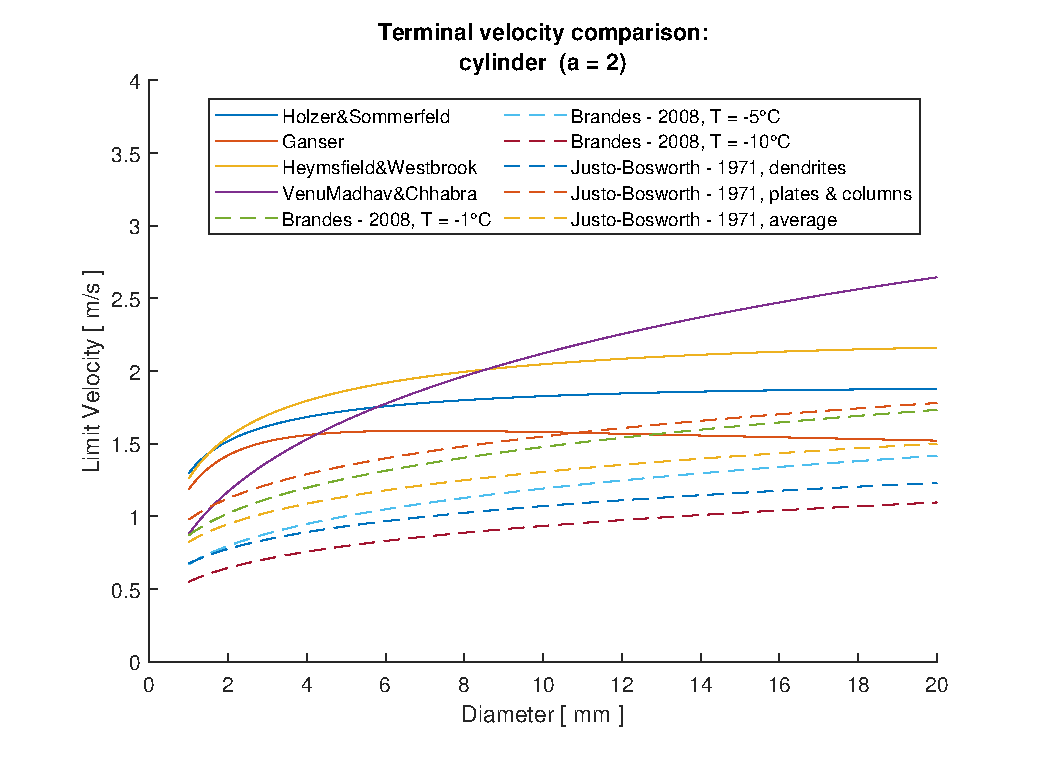
\includegraphics[height=\textheight,width=\textwidth,keepaspectratio] {vt_cylinder2.eps}		
	\end{frame}

	\begin{frame}{Terminal velocity - comparison}
		\centering
		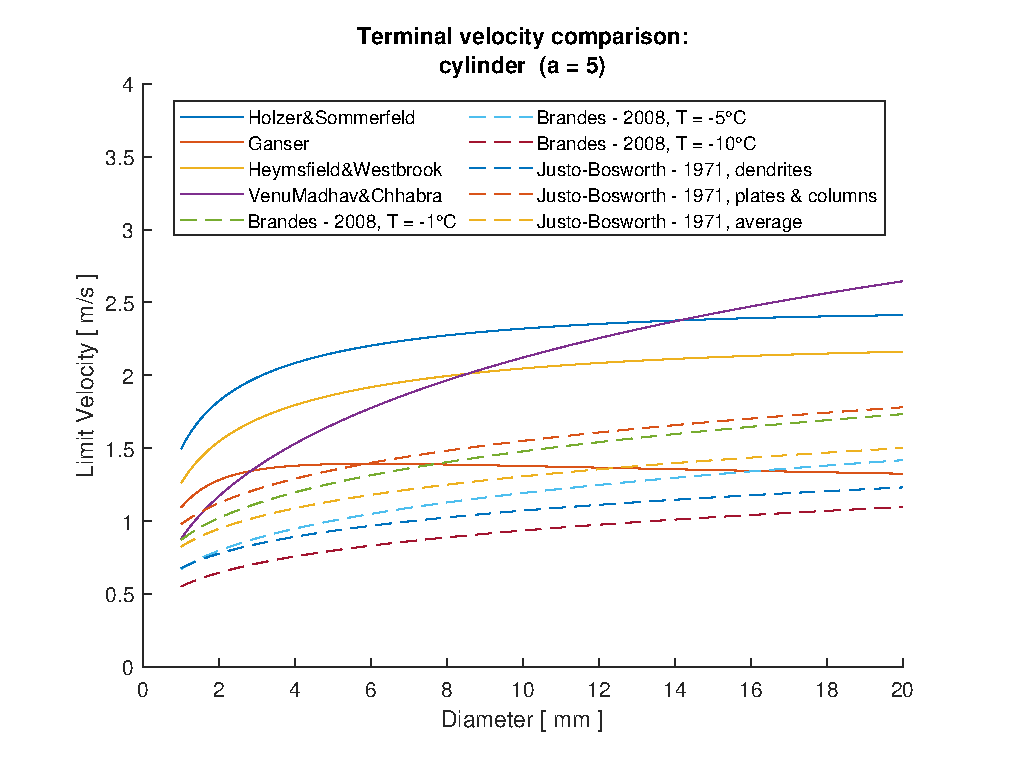
\includegraphics[height=\textheight,width=\textwidth,keepaspectratio] {vt_cylinder5.eps}		
	\end{frame}

	\begin{frame}{Range of Reynolds number - Camauli (2018)}
		\centering
		\includegraphics[height=\textheight,width=\textwidth,keepaspectratio] {Camauli.png}		
	\end{frame}

%	\begin{frame}{Recent work -- camera-based methods}
%		\begin{block}{China - 2017}
%			\centering
%			\includegraphics[width=\linewidth]{ComparisonChina.png}\\
%			\flushleft
%			Limitations: 
%			\begin{itemize}
%				\item Only three major regular particle shapes investigated (sphere, cube, cylinder)
%			\end{itemize}
%		\end{block}
%	\end{frame}
%
%	\begin{frame}{Recent work -- camera-based methods}
%		\begin{block}{Italy (Bari) - 2015}
%			\centering
%			\includegraphics[width=\linewidth]{ComparisonItaly.png}\\
%			\flushleft
%			Limitations:
%			\begin{itemize}
%				\item Small data sample
%				\item No comparison with Holzer and Sommerfeld (although good agreement with Ganser)
%			\end{itemize} 
%		\end{block}
%	\end{frame}
%
%	\begin{frame}{To do list}
%		\begin{itemize}
%			\item Read Loth-2008 (Snow??)
%			\item Replicate the work of the workshop on SU2
%			\item (Try the H\&S formula on the Italian data)
%		\end{itemize}
%	\end{frame}
\end{document}
